\section{Results}\label{sec:results}
Differences are mean paired differences in percentage points (pp) of gap to the reference cost; a negative value favors the first-named arm. Brackets give 95\% bootstrap intervals over instances, $p$ values are Holm-adjusted over the family of the study, and ``wins'' and ``losses'' count the instances (74 CVRPLIB, or 30 synthetic; 25 and 30 in Study 7; the sets of Studies 8--12 are given in their sections) on which the first-named arm has the lower and the higher mean gap. Every number, table and figure of this section is generated from the raw per-run files by scripts (Section~\ref{sec:verification}). All runs of Studies 1--6 and 8--12 were feasible; Study~7 has \num{s7_ninv} exclusions (Section~\ref{sec:s7}).

\subsection{Study 1: does the bandit beat chance?}\label{sec:s1}
Study~1 keeps the original loop (40 inner applications per step) and compares HG-UCB with uniform selection, UCB1, $\varepsilon$-greedy, probability matching and the classical GVNS at a matched budget (Table~\ref{tab:s1}; all contrasts in Table~\stab{tab:s1tests}).

\begin{table}[t]
\caption{Study 1: mean gap (\%) over 74 instances, original loop.}\label{tab:s1}
\centering
\small
\begin{adjustbox}{max width=\linewidth}
\begin{tabular}{lcc}
\toprule
Policy & $B=800$ & $B=4000$ \\
\midrule
Classical GVNS (fixed-order VND) & 3.00 & 2.29 \\
Uniform & 3.41 & 2.72 \\
UCB1 & 3.39 & 2.73 \\
Probability matching & 3.47 & 2.80 \\
HG-UCB (normalized) & 3.47 & 2.83 \\
$\varepsilon$-greedy & 3.50 & 2.86 \\
HG-UCB literal & 4.43 & 4.14 \\
\bottomrule
\end{tabular}
\end{adjustbox}
\end{table}


HG-UCB does not beat uniform selection: \num{s1d_hgucb_norm_uniforme_800}~pp \num{s1ci_hgucb_norm_uniforme_800} at $B=800$ (adjusted $p=\num{s1p_hgucb_norm_uniforme_800}$) and \num{s1d_hgucb_norm_uniforme_4000}~pp \num{s1ci_hgucb_norm_uniforme_4000} at $B=4000$ (adjusted $p=\num{s1p_hgucb_norm_uniforme_4000}$); nor does it differ significantly from UCB1, $\varepsilon$-greedy or probability matching (adjusted $p\ge\num{s1_minp_others_4000}$). The literal variant is \num{s1a_hgucb_literal_hgucb_norm_800}~pp \num{s1ci_hgucb_literal_hgucb_norm_800} and \num{s1a_hgucb_literal_hgucb_norm_4000}~pp \num{s1ci_hgucb_literal_hgucb_norm_4000} worse than normalized HG-UCB, losing on \num{s1l_hgucb_literal_hgucb_norm_800} and \num{s1l_hgucb_literal_hgucb_norm_4000} of 74 instances: the reward scale, not the policy, produces a loss larger than any difference among policies. The classical GVNS has the lowest mean gap and is significantly better than HG-UCB (\num{s1a_hgucb_norm_gvns_classico_800}~pp \num{s1ci_hgucb_norm_gvns_classico_800} and \num{s1a_hgucb_norm_gvns_classico_4000}~pp \num{s1ci_hgucb_norm_gvns_classico_4000}; HG-UCB is worse on \num{s1l_hgucb_norm_gvns_classico_800} and \num{s1l_hgucb_norm_gvns_classico_4000} of 74 instances), a difference examined in Study~2. Of the 12 pre-specified tests, \num{s1_nsig} are significant.

An exploratory run at $B=20\,000$ (\num{sub_n} instances, 5 seeds; low power) shows the same pattern (HG-UCB minus uniform \num{sub_d_hu_20000}~pp, interval containing zero).

\subsection{Study 2: where do the differences come from?}\label{sec:s2}
A diagnostic explains why the original loop is inefficient (all 74 instances, 10 seeds, $B=800$; exploratory). On average \num{diag_ultima}\% of its 40 inner applications per step occur after the last improvement of that step, and \num{diag_otimo}\% occur after all five operators have failed on the current solution (by instance, \num{diag_otimo_min}--\num{diag_otimo_max}\%), when, since every neighborhood is deterministic, no further application can change the solution. The original loop performs \num{sh_f40_800} shakes within 800 applications; random order with local-optimum termination performs \num{sh_ubestlo_800} on average. Study~2 decomposes the structure by crossing operator \emph{order} (fixed or uniformly random), \emph{acceptance} (\textit{best} or \textit{shaken}) and inner-loop \emph{termination} (local optimum, LO, or 40 applications, F40) (Table~\ref{tab:s2a}; all contrasts in Table~\stab{tab:s2tests}).

\begin{table}[t]
\caption{Study 2A: mean gap (\%) over 74 instances by search structure (five operators).}\label{tab:s2a}
\centering
\small
\begin{adjustbox}{max width=\linewidth}
\begin{tabular}{lccc}
\toprule
Order / acceptance / termination & $B=800$ & $B=4000$ & Role \\
\midrule
Random / best / LO & 2.66 & 1.92 & best structure \\
Random / shaken / LO & 2.88 & 2.10 &  \\
Fixed / best / LO & 3.00 & 2.29 & classical GVNS \\
Fixed / shaken / LO & 3.18 & 2.58 &  \\
Random / best / F40 & 3.32 & 2.53 &  \\
Random / shaken / F40 & 3.41 & 2.72 & original loop, uniform \\
\bottomrule
\end{tabular}
\end{adjustbox}
\end{table}


\emph{Termination} is the dominant factor. Stopping at a local optimum instead of running 40 applications improves the gap by \num{g_term_abs}~pp across the two acceptance rules and two budgets (better on \num{g_term_w} of 74 instances; adjusted $p<10^{-4}$ in all four contrasts). \emph{Acceptance} contributes \num{g_acc_abs}~pp (all four contrasts significant, the weakest at adjusted $p=\num{s2p_C3_4000}$; descriptively the effect concentrates in set X, Table~\stab{tab:s2set}). Contrary to our pre-specified expectation, \emph{random order beats fixed order} by \num{g_ord_best_abs}~pp under \textit{best} acceptance and \num{g_ord_shaken_abs}~pp under \textit{shaken}, significantly at both budgets: the fixed order always restarts from 2-Opt, which then absorbs \num{s2_2opt_share_fixed_4000}--\num{s2_2opt_share_fixed_800}\% of all applications. Moving from the original loop to random order, \textit{best} acceptance and LO termination reduces the gap from \num{s2a_gap_uniforme_4000}\% to \num{s2a_gap_s2a_U_best_LO_4000}\% at $B=4000$ with no learning at all.

\paragraph{AOS inside the efficient structure}
In the best structure (\textit{best}/LO, selecting among operators not yet failed) we compare four adaptive policies with random order (rows D1--D4 of Table~\stab{tab:s2tests}). Probability matching ties with random order at both budgets, and UCB1 does at $B=800$ (\num{s2d_D1_800}~pp \num{s2ci_D1_800}); at $B=4000$ UCB1 is marginally worse (\num{s2d_D1_4000}~pp \num{s2ci_D1_4000}, adjusted $p=\num{s2p_D1_4000}$), a difference whose two-level interval \num{rb2_E2_4000_s2b_ucb1_s2a_U_best_LO} includes zero. $\varepsilon$-greedy and HG-UCB are significantly \emph{worse} at both budgets, a result that survives the two-level bootstrap (95\% intervals \num{rb2_E2_800_s2b_eps_greedy_s2a_U_best_LO} and \num{rb2_E2_4000_s2b_eps_greedy_s2a_U_best_LO} for $\varepsilon$-greedy; \num{rb2_E2_800_s2b_hgucb_norm_s2a_U_best_LO} and \num{rb2_E2_4000_s2b_hgucb_norm_s2a_U_best_LO} for HG-UCB). Adaptive policies are better than the classical fixed order by \num{g_vsfixed_abs}~pp, but this reflects the order effect above, not adaptation. Of the 28 pre-specified tests, \num{s2_nsig} are significant.

\subsection{Study 3: a larger, heterogeneous operator pool}\label{sec:s3}
With five similar deterministic operators there may be no room for adaptation. We therefore add 2-opt*, Or-opt (segments of 2--3), an intra-route swap, CROSS exchange (segments up to 3) and a naive SWAP* \citep{vidal2022}, for a pool of ten. The cost of an application differs by a factor of \num{eff_cost_ratio} across operators (mean \num{eff_cost_0}k distance evaluations for 2-Opt, \num{eff_cost_9}k for SWAP*; Table~\ref{tab:eff}) and the budget is therefore measured in distance evaluations (Section~\ref{sec:budgets}). We cross two stopping rules---LO, where adaptation can only reorder, and R5 (stop after five consecutive failures, sampling with replacement), where it can avoid costly useless operators---with five policies (Section~\ref{sec:policies}). Of the 34 pre-specified tests, \num{s3_nsig} are significant (\num{s3_nsig_E1} at $E_1$, \num{s3_nsig_E2} at $E_2$; Table~\ref{tab:s3}; all contrasts in Table~\stab{tab:s3tests}).

\begin{table}[t]
\caption{Study 3: mean gap (\%) over 74 instances (budgets $E_1$ and $E_2$); the last two rows use the original five operators with the same budget.}\label{tab:s3}
\centering
\small
\begin{adjustbox}{max width=\linewidth}
\begin{tabular}{lcc}
\toprule
Arm & $E_1$ & $E_2$ \\
\midrule
R5, UCB1 (cost-aware) & 2.10 & 1.33 \\
R5, uniform & 2.19 & 1.36 \\
R5, probability matching (cost-aware) & 2.19 & 1.40 \\
LO, uniform & 2.23 & 1.42 \\
LO, probability matching (cost-aware) & 2.25 & 1.43 \\
LO, UCB1 (cost-aware) & 2.26 & 1.45 \\
LO, HG-UCB (cost-aware) & 2.34 & 1.56 \\
R5, HG-UCB (cost-aware) & 2.15 & 1.56 \\
LO, fixed order by cost & 2.37 & 1.62 \\
\addlinespace
R5, fixed order by cost & 2.16 & 1.63 \\
Five operators, LO, uniform & 2.74 & 1.96 \\
Five operators, LO, fixed order & 2.99 & 2.30 \\
\bottomrule
\end{tabular}
\end{adjustbox}
\end{table}


\emph{The larger pool is the only large effect:} with the same stopping rule and random order, ten operators beat five by \num{s3a_T1_1}~pp \num{s3ci_T1_1} and \num{s3a_T1_5}~pp \num{s3ci_T1_5} at $E_1$ and $E_2$ (better on \num{s3w_T1_1} and \num{s3w_T1_5} of 74 instances; adjusted $p<10^{-4}$), in all four instance sets (Table~\stab{tab:s3set}). Random order again beats the classical fixed order for the original pool (\num{s3a_T3_1} and \num{s3a_T3_5}~pp). A fixed order \emph{by cost} is worse than random order with the large pool (\num{s3d_LO_FOCvsU_1} and \num{s3d_LO_FOCvsU_5}~pp under LO; \num{s3d_R5_FOCvsU_5}~pp under R5 at $E_2$). \emph{No adaptive policy beats uniform selection:} UCB1 and probability matching tie with it under both stopping rules and budgets, and HG-UCB is significantly worse at $E_2$ (\num{s3d_LO_hgucbcvsU_5}~pp \num{s3ci_LO_hgucbcvsU_5} under LO, \num{s3d_R5_hgucbcvsU_5}~pp \num{s3ci_R5_hgucbcvsU_5} under R5). UCB1 and probability matching do beat the fixed order by cost at $E_2$ (by \num{g_s3_vsfoc_abs}~pp), which reflects the weakness of that order. The cost-aware reward made no measurable difference to HG-UCB (\num{rbd_E3_1_s3_R5_hgucbc_s3_R5_hgucb_cego} and \num{rbd_E3_5_s3_R5_hgucbc_s3_R5_hgucb_cego}~pp at $E_1$ and $E_2$, intervals \num{rb1_E3_1_s3_R5_hgucbc_s3_R5_hgucb_cego} and \num{rb1_E3_5_s3_R5_hgucbc_s3_R5_hgucb_cego}). The stopping rule (R5 versus LO) has no detectable effect under random order (\num{s3d_T2_1} and \num{s3d_T2_5}~pp, not significant).

Uniform and adaptive policies spend \num{s3_swap_min}--\num{s3_swap_max}\% of their distance evaluations in SWAP* (the fixed order by cost, \num{s3_swap_foc_min}--\num{s3_swap_foc_max}\%), with HG-UCB concentrating the most (\num{s3_swap_hg_lo}\% under LO; Figure~S3 of the supplement). This concentration is a cost effect, not an efficiency one: SWAP* has the highest success rate per application (\num{eff_suc_9}\%) but the lowest relative gain per thousand distance evaluations, \num{eff_ratio} times below 2-Opt (Table~\ref{tab:eff}). Whether the benefit of the larger pool comes from the cheap or from the expensive additions is tested in Study~5.

\begin{table}[t]
\caption{Efficiency of each operator under uniform selection (R5, ten operators, $E_1$, 74 instances, 10 seeds): success rate per application, mean relative gain per success, mean cost per application (thousand distance evaluations) and relative gain (\%) per thousand distance evaluations, sorted by the last column.}\label{tab:eff}
\centering
\small
\begin{adjustbox}{max width=\linewidth}
\begin{tabular}{lcccc}
\toprule
Operator & Success (\%) & Gain/success (\%) & Cost (k eval.) & Gain per 1k eval. (\%) \\
\midrule
2-Opt & 37.3 & 1.10 & 1.1 & 0.364 \\
Move(1) & 38.7 & 1.06 & 1.9 & 0.219 \\
2-opt* & 24.3 & 1.45 & 1.8 & 0.192 \\
Swap-intra & 30.3 & 1.07 & 2.0 & 0.166 \\
Reloc(1,0) & 33.4 & 1.50 & 4.5 & 0.111 \\
Or-opt(2-3) & 37.2 & 1.23 & 5.2 & 0.088 \\
Reloc(2,0) & 10.6 & 2.34 & 3.8 & 0.065 \\
Swap(1,1) & 24.4 & 1.51 & 18.9 & 0.019 \\
CROSS & 21.5 & 1.48 & 24.7 & 0.013 \\
SWAP* & 40.0 & 1.55 & 70.9 & 0.009 \\
\bottomrule
\end{tabular}
\end{adjustbox}
\end{table}


\subsection{Study 4: tuned policies, a tuned static mixture and independent instances}\label{sec:s4}
Study~4 gives adaptation its best chance and measures the headroom. The hyperparameters of UCB1, probability matching and HG-UCB were tuned with one protocol (24 synthetic tuning instances disjoint from the evaluation instances, R5 structure at $E_1$, five seeds common to all configurations, grids of 5, 9 and 9 points; Section~7 of the online supplement), and a \emph{static mixture}---a fixed probability vector over the ten operators, with no learning---was tuned on the same instances by a $(1{+}4)$ evolution strategy (61 evaluations; weights in Table~\stab{tab:s4pesos}). Table~\stab{tab:s4config} lists the selected values. The gains of tuning on the tuning set are small for the three policies (\num{s4_tune_ucb1_d}\% to \num{s4_tune_ucb1_t}\% for UCB1, \num{s4_tune_pm_d}\% to \num{s4_tune_pm_t}\% for probability matching, \num{s4_tune_hgucb_d}\% to \num{s4_tune_hgucb_t}\% for HG-UCB) and of the order of the tuning noise: uniform selection implemented as an equal-weight static mixture differs from the uniform-selection arm by \num{s4_tune_noise}~pp on the same instances (different consumption of random numbers). The tuned static mixture, by contrast, improves the tuning-set gap from \num{s4_tune_static0}\% (equal weights) to \num{s4_tune_static_best}\%.



On the 74 CVRPLIB instances (Table~\stab{tab:s4tests}), \emph{no tuned policy beats uniform selection}: UCB1 \num{s4d_V1_1} and \num{s4d_V1_5}~pp, probability matching \num{s4d_V2_1} and \num{s4d_V2_5}~pp at $E_1$ and $E_2$ (no test significant), and tuned HG-UCB is significantly worse at $E_2$ (\num{s4d_V3_5}~pp \num{s4ci_V3_5}, adjusted $p=\num{s4p_V3_5}$). The improvement on the tuning set does not transfer: tuned UCB1 is no better than its default on CVRPLIB (\num{s4_gap_ucb1_t_1}\% against \num{s4_gap_ucb1_d_1}\% at $E_1$, \num{s4_gap_ucb1_t_5}\% against \num{s4_gap_ucb1_d_5}\% at $E_2$), as expected when the best of several noisy evaluations is selected. The \emph{static mixture} is at best marginally better than uniform selection: \num{s4d_V4_1}~pp \num{s4ci_V4_1} at $E_1$ (adjusted $p=\num{s4p_V4_1}$) and \num{s4d_V4_5}~pp \num{s4ci_V4_5} at $E_2$. Even with a distribution tuned offline on 24 instances, the gain over uniform selection is \num{s4a_V4_1}~pp at the smaller budget (not significant after correction) and null at the larger one, a benchmark for what a single global operator distribution can add. No tuned policy beats the static mixture (\num{s4d_V5_1}, \num{s4d_V6_1} and \num{s4d_V7_1}~pp at $E_1$ for UCB1, probability matching and HG-UCB; probability matching is significantly worse, adjusted $p=\num{s4p_V6_1}$). Of the 14 tests, \num{s4_nsig74} are significant, and in both the adaptive policy is the worse arm.

The learned mixture concentrates \num{s4_wp_2opt_pair}\% of its probability on 2-Opt and 2-opt*, two of the cheapest and most efficient operators, and only \num{s4_wp_expensive}\% on the three expensive ones, Swap(1,1), CROSS and SWAP* (Table~\stab{tab:s4pesos}), consistent with the per-evaluation efficiencies of Table~\ref{tab:eff}; it gives SWAP* only \num{s4_wp9}\% of its selections (although SWAP* absorbs \num{s4_static_swap_1}\% of its evaluations because of its cost), so the pool benefit does not require frequent use of the most expensive operator.

On the 30 synthetic validation instances (up to 300 customers, 5 seeds, $E_1$; Table~\stab{tab:s4val}) the pool effect replicates (\num{s4d_W1}~pp \num{s4ci_W1}, adjusted $p<10^{-4}$), whereas the effect of the fixed order by cost does not (\num{s4d_W2}~pp, adjusted $p=\num{s4p_W2}$) and no tuned policy differs from uniform selection (UCB1 \num{s4d_W3}, probability matching \num{s4d_W4}, HG-UCB \num{s4d_W5}~pp). The static mixture is \num{s4d_W6}~pp \num{s4ci_W6} from uniform selection (adjusted $p=\num{s4p_W6}$). Of the 6 tests, \num{s4_nsigval} is significant.

\subsection{Study 5: which operators explain the pool effect?}\label{sec:s5}
Table~\ref{tab:eff} suggests that the cheap operators are far more efficient than the expensive ones, so we expected the cheap additions to explain the benefit of the larger pool. Study~5 tests this with uniform selection on subsets of the pool (Table~\stab{tab:s5}): P8c adds 2-opt*, Or-opt and Swap-intra to the original five (P5), P7e adds CROSS and SWAP*, and P7c removes Swap(1,1), CROSS and SWAP* from the ten. \emph{The expectation is refuted:} the expensive pair is at least as valuable as the cheap trio. Adding the three cheap operators improves the gap by \num{g_s5_A1}~pp (range over the two stopping rules and the two budgets), whereas adding only CROSS and SWAP* improves it by \num{g_s5_A2}~pp and recovers \num{s5_rec_P7e_rng}\% of the effect of the full pool, against \num{s5_rec_P8c_rng}\% for the cheap trio (A1 and A2: all eight tests significant; Table~\stab{tab:s5tests}). The expensive operators still add value on top of the cheap ones (A3, \num{g_s5_A3}~pp, significant in \num{s5_A3_nsig} of 4 cases), removing Swap(1,1), CROSS and SWAP* from the ten operators costs \num{g_s5_A4}~pp (A4, significant in \num{s5_A4_nsig} of 4 cases), and even removing only Swap(1,1) from the eight-operator pool costs \num{g_s5_A5}~pp (A5, significant in \num{s5_A5_nsig} of 4 cases). Of the 20 pre-specified tests, \num{s5_nsig} are significant.


The operators that Table~\ref{tab:eff} ranks as least efficient therefore contribute substantially. Under uniform selection SWAP* absorbs \num{s5_p7e_swap_1}\% of the distance evaluations in P7e (CROSS \num{s5_p7e_cross_1}\%), and the tuned static mixture of Study~4 reaches a gap not significantly different from that of uniform selection over the ten operators while spending \num{s4_static_swap_1}\% of its evaluations on SWAP* instead of \num{s3_U_swap_1}\%. The per-evaluation efficiency measured under uniform selection thus understates the value of costly operators. A direct, exploratory diagnostic explains why: at \num{compl_n} local optima of the five original operators (74 instances, 3 seeds, 8 local optima each, reached by a fixed-order descent after a shake), one application of the best-improvement move of SWAP* finds an improvement in \num{compl_swapstar}\% of the cases and CROSS in \num{compl_cross}\%, against \num{compl_2opt}\% for 2-opt*, \num{compl_oropt}\% for Or-opt and \num{compl_swapintra}\% for Swap-intra; in \num{compl_so_caros}\% of the local optima only CROSS or SWAP* find an improvement, and in \num{compl_so_baratos}\% only the cheap added operators do. The expensive operators are complementary to the original ones: they improve solutions on which the cheap neighborhoods have failed.

\subsection{Study 6: further policy families and contextual policies}\label{sec:s6}
Study~6 asks whether the null results are specific to the four policy families examined so far. In the structure of Study~4 (R5, ten operators) and without tuning, we add EXP3, Thompson sampling, sliding-window UCB, adaptive pursuit, an efficiency UCB that charges the cost of every application (two exploration constants) and two contextual Thompson policies (Section~\ref{sec:policies}; Table~\ref{tab:s6}).

\inputopt{tab_s6}

\emph{No policy beats uniform selection:} none of the 16 pre-specified tests shows an improvement, and in \num{s6_nsig} of them the policy is significantly worse (Table~\ref{tab:s6}). EXP3 and sliding-window UCB are indistinguishable from uniform selection at both budgets (EXP3 \num{s6d_W1_1} and \num{s6d_W1_5}~pp, sliding-window UCB \num{s6d_W3_1} and \num{s6d_W3_5}~pp at $E_1$ and $E_2$). Thompson sampling and adaptive pursuit are worse (\num{s6d_W2_1} and \num{s6d_W2_5}~pp; \num{s6d_W4_1} and \num{s6d_W4_5}~pp), and so are the two contextual policies at $E_2$ (\num{s6d_W7_5} and \num{s6d_W8_5}~pp). The policy that charges the cost of every application is the worst of the study: with $C=1$ it is \num{s6d_W5_1} and \num{s6d_W5_5}~pp worse than uniform selection at $E_1$ and $E_2$, and with $C=2$ it is \num{s6d_W6_5}~pp worse at $E_2$. It does what it is designed to do, moving evaluations to cheap operators (at $E_2$, 2-Opt receives \num{s6_eff_2opt_5}\% of its evaluations and SWAP* \num{s6_eff_swap_5}\%, against \num{s3_U_2opt_5}\% and \num{s3_U_swap_5}\% under uniform selection), and, in line with Study~5, it loses because the expensive operators are worth more than their measured efficiency suggests. On the 30 synthetic validation instances (exploratory, $E_1$, no multiplicity correction) \num{s6v_nworse_raw} of the eight arms are nominally worse than uniform selection and one, sliding-window UCB, is nominally better (\num{s6vd_3}~pp \num{s6vci_3}, unadjusted $p=\num{s6vp_3}$); this difference does not survive a Holm correction over the eight comparisons (adjusted $p=\num{s6vph_3}$) and is not seen on CVRPLIB (\num{s6d_W3_1} and \num{s6d_W3_5}~pp).

\subsection{Study 7: adaptive move selection inside HGS-CVRP}\label{sec:s7}
Study~7 asks whether the null results hold inside a state-of-the-art local search (Section~\ref{sec:hgsaos}; Table~\ref{tab:s7}). They do, but the test is weak, because within HGS-CVRP the order in which the moves of a node pair are tried hardly matters. None of the 20 pre-specified tests is significant, the largest difference in absolute value is \num{s7_maxabs}~pp (\num{s7_maxabs_adapt}~pp for adaptive policies), and the original order does not differ significantly from the uniform random order either (on the synthetic instances at 250 generations it is \num{s7a_fixed_P2_250}~pp worse, interval \num{s7ci_fixed_P2_250}, whose lower limit is above zero, but the Wilcoxon test gives raw $p=\num{s7pr_fixed_P2_250}$). The minimum detectable effect at 80\% power is \num{s7_mde_med}~pp (median over the 20 tests). Of the 16 contrasts of adaptive policies at the primary checkpoints, \num{s7_neq} are equivalent to the random order within $\pm0.05$~pp, and so are all \num{s7_late_n} contrasts at 2000 and 4000 generations (exploratory). Including the \num{s7_ninv} runs excluded for violating the route-count bound of our convention (all on one instance, X-n195-k51) changes nothing (\num{s7_sens_nsig} significant tests). There is structure to learn, since the success rate per attempt varies by a factor of \num{s7_succ_ratio} across move types (from \num{s7_succ_2} to \num{s7_succ_4} improving moves per $10^4$ attempts under the random order), but because the first improving move is applied and a pair rarely admits several, ordering has little leverage, as a comment in the HGS-CVRP code notes. Budgets are matched in generations, not in CPU time: a generation takes \num{s7_cpu_fixed}~ms of CPU with the original order, \num{s7_cpu_unif}~ms with the uniform random order and \num{s7_cpu_ts}--\num{s7_cpu_hg}~ms with Thompson sampling to HG-UCB (probability matching, \num{s7_cpu_pm}~ms, suffers from floating-point underflow of its estimates, an implementation artifact). The original order is the fastest, so at equal CPU time it would beat every learned order, whereas the cost differences among the learned and random orders reflect our implementation. Because even randomizing the order changes so little, the study shows that nothing is gained at this decision point of HGS-CVRP; it is not evidence about other decision points of the solver.

\inputopt{tab_s7}

\subsection{Study 8: a positive control with planted useless operators}\label{sec:s8}
The null results above could reflect an insensitive protocol rather than the absence of exploitable structure. Study~8 (Section~\ref{sec:s8design}) adds four useless operators to the pool. Under uniform selection they absorb \num{s8_duds_D4x4_U}\% and \num{s8_duds_D4x8_U}\% of the distance evaluations and raise the gap by \num{s8_loss_D4x4}~pp and \num{s8_loss_D4x8}~pp (Table~\ref{tab:s8}). Of the 12 pre-specified tests, \num{s8_nsig} are significant, all in favor of the adaptive policy, so the protocol is not blind: Thompson sampling is \num{s8a_D4x8_ts}~pp better than uniform selection in the $8n^2$ pool (\num{s8ci_D4x8_ts}, adjusted $p=\num{s8p_D4x8_ts}$), the efficiency UCB \num{s8a_D4x8_eff}~pp (\num{s8ci_D4x8_eff}, $p=\num{s8p_D4x8_eff}$) and the cost-aware HG-UCB \num{s8a_D4x8_hgucbc}~pp ($p=\num{s8p_D4x8_hgucbc}$); in the $4n^2$ pool only UCB1 is significant (\num{s8a_D4x4_ucb1c}~pp, $p=\num{s8p_D4x4_ucb1c}$).

\begin{table}[t]
\caption{Study 8 (positive control): mean gap (\%) over 74 instances at $E_1$ in the clean pool of ten operators and in pools with four planted useless operators (each costing $4n^2$ or $8n^2$ distance evaluations and never improving); in parentheses, the difference from uniform selection \emph{in the same pool} in pp (* marks Holm-significance over the 12 confirmatory tests; clean-pool comparisons are exploratory).}\label{tab:s8}
\centering
\small
\begin{adjustbox}{max width=\linewidth}
\begin{tabular}{lccc}
\toprule
Policy & Clean pool & 4 useless, $4n^2$ & 4 useless, $8n^2$ \\
\midrule
Uniform selection & 2.19 & 2.55 & 2.72 \\
UCB1 (cost-aware) & 2.10 ($-$0.08) & 2.48 ($-$0.07*) & 2.67 ($-$0.05) \\
Probability matching (cost-aware) & 2.19 ($+$0.01) & 2.48 ($-$0.07) & 2.68 ($-$0.05) \\
HG-UCB (cost-aware) & 2.15 ($-$0.04) & 2.54 ($-$0.01) & 2.65 ($-$0.07*) \\
Thompson sampling & 2.32 ($+$0.14) & 2.43 ($-$0.12) & 2.51 ($-$0.22*) \\
EXP3 & 2.19 ($+$0.01) & 2.54 ($-$0.01) & 2.74 ($+$0.01) \\
Efficiency UCB & 2.48 ($+$0.29) & 2.50 ($-$0.05) & 2.56 ($-$0.16*) \\
\bottomrule
\end{tabular}
\end{adjustbox}
\end{table}


The policies differ sharply in how much of the planted loss they recover (exploratory; Table~\stab{tab:s8rec}). The efficiency UCB recovers \num{s8rec_D4x8_eff}\% of it in the $8n^2$ pool (interval \num{s8reci_D4x8_eff}) and Thompson sampling \num{s8rec_D4x8_ts}\% (\num{s8reci_D4x8_ts}), cutting the share of evaluations wasted on useless operators from \num{s8_duds_D4x8_U}\% to \num{s8_duds_D4x8_eff}\% and \num{s8_duds_D4x8_ts}\%; UCB1, probability matching, HG-UCB and EXP3 with default hyperparameters recover at most \num{s8rec_D4x8_pmc}\%, and keep spending \num{s8_duds_D4x8_hgucbc}--\num{s8_duds_D4x8_exp3}\% of the evaluations on the useless operators. For probability matching a structural reason is the exploration floor: with $p_{\min}=0.05$ and $k=10$ or 14 operators, 50\% or 70\% of the probability mass is reserved for uniform selection. Insurance has a premium: in the clean pool Thompson sampling and the efficiency UCB are significantly worse than uniform selection (\num{s8d_P10_ts} and \num{s8d_P10_eff}~pp, exploratory), and even the best policy in an inflated pool stays above uniform selection in the clean pool, so the best defense against a bad pool remains not to build one. The ceiling of what a policy can protect is itself small, because of diminishing returns of the budget: wasting \num{s8_duds_D4x8_U}\% of the evaluations costs only \num{s8_loss_D4x8}~pp.

\subsection{Study 9: adaptive selection in a stochastic large-neighborhood search}\label{sec:s9}
Study~9 (Section~\ref{sec:s9design}) is the first setting in which adaptive selection helps. The adaptive weights of Ropke and Pisinger are \num{s9prim_a}~pp better than uniform selection on the \num{s9_n_inst} instances (\num{s9prim_ci}; \num{s9prim_w} wins and \num{s9prim_l} losses; $p<10^{-4}$ in the single primary test), which lowers the mean gap from \num{s9_gap_U}\% to \num{s9_gap_RP}\% (Table~\ref{tab:s9}). Of the 12 secondary tests, \num{s9_nbetter} favor the adaptive policy after Holm correction: probability matching with the tuned $\gamma=0.05$ (\num{s9d_pm_X}~pp on set X and \num{s9d_pm_V}~pp on the synthetic set), EXP3 (\num{s9d_exp3_X} and \num{s9d_exp3_V}~pp) and HG-UCB on set X (\num{s9d_hgucb_X}~pp). UCB1 does not differ from uniform selection, and Thompson sampling and the efficiency UCB are much worse (\num{s9d_ts_V} and \num{s9d_eff_X}~pp on the sets where they are significant). The usage statistics show the mechanism: RP, UCB1 and probability matching move the repair choice to regret-2 (\num{s9_reg2_RP}\%, \num{s9_reg2_ucb1}\% and \num{s9_reg2_pm}\% of the repair choices, against \num{s9_reg2_U}\% under uniform selection), the operator that dominates the other two here. This heterogeneity of quality, which the best-improvement operators of the VNS do not have, is what the policies exploit, in line with the positive control of Study~8; the same two policies that were best against useless operators (Thompson sampling, the efficiency UCB) concentrate too early on the cheap or random operators and lose, so the choice of policy depends on the kind of heterogeneity.

\begin{table}[t]
\caption{Study 9 (ALNS with stochastic destroy and repair operators, $1500\,n^2$ distance evaluations): mean gap (\%) on the 21 instances of set X (ten seeds) and the 30 synthetic validation instances (five seeds); in parentheses, the difference from uniform selection in pp (* marks Holm-significance over the 12 secondary tests; for the adaptive weights, the primary test on the 51 instances is in the text and the per-set differences are exploratory). The last rows are VNS arms at the same budget.}\label{tab:s9}
\centering
\small
\begin{adjustbox}{max width=\linewidth}
\begin{tabular}{lcc}
\toprule
Policy & Set X & Synthetic validation \\
\midrule
Uniform selection & 1.48 & 1.86 \\
Adaptive weights (Ropke--Pisinger) & 1.24 ($-$0.24) & 1.42 ($-$0.44) \\
UCB1 & 1.74 ($+$0.26) & 2.20 ($+$0.34) \\
Probability matching & 1.15 ($-$0.33*) & 1.40 ($-$0.46*) \\
HG-UCB & 1.31 ($-$0.16*) & 1.60 ($-$0.26) \\
Thompson sampling & 2.63 ($+$1.16) & 3.04 ($+$1.18*) \\
EXP3 & 1.21 ($-$0.27*) & 1.52 ($-$0.34*) \\
Efficiency UCB & 3.45 ($+$1.97*) & 3.81 ($+$1.95*) \\
VNS, uniform selection (same budget) & 3.15 & 2.92 \\
VNS, static mixture (same budget) & 2.72 & 2.58 \\
\bottomrule
\end{tabular}
\end{adjustbox}
\end{table}


The search structure matters more than the selection layer: at the same budget, ALNS with uniform selection is better than VNS with uniform selection by \num{s9ta_vns_U_X} (set X) and \num{s9ta_vns_U_V}~pp (synthetic set), and better than VNS with the tuned static mixture by \num{s9ta_vns_static_X} and \num{s9ta_vns_static_V}~pp (Holm-adjusted $p\le0.002$ in the four tests). Two cautions apply. The gains of the adaptive policies are two to three times the average adaptive layer of the ALNS literature, and a fixed probability vector tuned offline might capture the same gain, since it can also learn that regret-2 is the best repair; this control is the object of Study~12 (Section~\ref{sec:s12}).

\subsection{Study 12: is the gain of the ALNS adaptation?}\label{sec:s12res}
It is not (Section~\ref{sec:s12}; Table~\ref{tab:s12}). A static mixture tuned offline (destroy probabilities \num{s12_wd_0}, \num{s12_wd_1}, \num{s12_wd_2} and \num{s12_wd_3}\% for random, worst, related and route removal; repair probabilities \num{s12_wr_0}, \num{s12_wr_1} and \num{s12_wr_2}\% for greedy, regret-2 and the cheap repair) is \num{s12a_static_U}~pp better than uniform selection (\num{s12ci_static_U}, adjusted $p<10^{-3}$), and the adaptive weights do not differ from it (\num{s12d_RP_static}~pp, \num{s12ci_RP_static}, adjusted $p=\num{s12p_RP_static}$); the static mixture captures \num{s12cap_static}\% of the gain of the adaptive weights over uniform selection (interval \num{s12capci_static}), and probability matching, the best adaptive arm, is \num{s12d_pm_static}~pp from it (adjusted $p=\num{s12p_pm_static}$). The simplest control does best: always using the regret-2 repair, with uniform destroy, is \num{s12a_reg2_U}~pp better than uniform selection and \num{s12a_RP_reg2}~pp \emph{better} than the adaptive weights (\num{s12ci_RP_reg2}; adjusted $p=\num{s12p_RP_reg2}$), the price of having to learn which repair is the best.

\begin{table}[t]
\caption{Study 12 (static control for the ALNS): mean gap (\%) on set X (21 instances), the synthetic validation set (30) and both (51), and the difference from uniform selection over the 51 instances in pp. The static mixture and the fixed repair are new arms; the other rows are the corresponding arms of Study 9 (same code, instances and seeds).}\label{tab:s12}
\centering
\small
\begin{adjustbox}{max width=\linewidth}
\begin{tabular}{lcccc}
\toprule
Policy & Set X & Synthetic & All & Difference \\
\midrule
Uniform selection & 1.48 & 1.86 & 1.70 \\
Static mixture (tuned offline) & 1.16 & 1.45 & 1.33 & $-$0.37 \\
Fixed repair: always regret-2 & 1.16 & 1.29 & 1.23 & $-$0.47 \\
Adaptive weights (Ropke--Pisinger) & 1.24 & 1.42 & 1.34 & $-$0.36 \\
Probability matching (tuned) & 1.15 & 1.40 & 1.30 & $-$0.40 \\
\bottomrule
\end{tabular}
\end{adjustbox}
\end{table}


The gain of Study~9 is therefore a gain from weighting the operators well, not from adapting during the run. What the adaptive policies provide is that discovery without tuning: the adaptive weights reach the level of the tuned mixture with no tuning run, whereas the mixture needed \num{s12_tune_runs} tuning runs (and a tuning gap of \num{s12_tune_gap}\% against \num{s12_tune_eq}\% for equal weights). This is consistent with the tuned static mixture of Study~4 and with Study~10, where no policy ever beat the best fixed configuration, and it sharpens the conclusion of the paper: adaptation recovers a good fixed configuration when none is available, but we found no setting in which it exceeds one.

\subsection{Study 10: larger instances}\label{sec:s10}
The pattern that motivated Study~10 does not replicate (Section~\ref{sec:s10design}; Table~\ref{tab:s10}). On the \num{s10_n_inst} new instances of 200 to 500 customers no mixture or policy is significantly better than uniform selection after correction: the mixture of Study~4 is \num{s10a_static_S}~pp better (\num{s10ci_static_S}; unadjusted $p=\num{s10pr_static_S}$, adjusted $p=\num{s10p_static_S}$) and the mixture tuned at this size \num{s10a_static_L}~pp better (\num{s10ci_static_L}; adjusted $p=\num{s10p_static_L}$), with a minimum detectable effect of \num{s10mde_static_L}--\num{s10mde_static_S}~pp at 80\% power; the three cost-aware online policies are within \num{s10a_ucb1c}~pp of uniform selection, and Thompson sampling and the efficiency UCB are significantly \emph{worse} (\num{s10d_ts} and \num{s10d_eff}~pp). The advantage of the mixtures does not grow with $n$: for the mixture tuned at this size it is \num{s10dn200_static_L}, \num{s10dn300_static_L}, \num{s10dn400_static_L} and \num{s10dn500_static_L}~pp at 200, 300, 400 and 500 customers (Spearman correlation with $n$ \num{s10rho_static_L}, $p=\num{s10rhop_static_L}$, the wrong sign for the hypothesis). The naive SWAP* absorbs \num{s10_swap_n200}--\num{s10_swap_n500}\% of the evaluations under uniform selection, so these instances are a demanding setting for any policy, yet tuning on them (gap \num{s10_tune_gap_eq}\% with equal weights, \num{s10_tune_gap_L}\% after the search) did not transfer. We conclude that the subgroup pattern of the earlier data was a selection effect, and that a mixture learned offline yields at best a few tenths of a point, with large variance.

\begin{table}[t]
\caption{Study 10: instances of 200 to 500 customers (20 synthetic validation instances, five seeds, $E_1$): mean gap (\%), mean paired difference from uniform selection in pp [95\% CI], unadjusted $p$ and Holm-adjusted $p$ over seven tests.}\label{tab:s10}
\centering
\small
\begin{adjustbox}{max width=\linewidth}
\begin{tabular}{lcccc}
\toprule
Policy & Gap & Difference & $p$ & $p$ (Holm) \\
\midrule
Uniform selection & 4.44 & & &  \\
Static mixture tuned at $n\le150$ (Study 4) & 4.04 & $-$0.40 [$-$0.69, $-$0.13] & 0.027 & 0.13 \\
Static mixture tuned at $n=200$--400 & 4.30 & $-$0.14 [$-$0.25, $-$0.04] & 0.030 & 0.13 \\
UCB1 (cost-aware) & 4.35 & $-$0.09 [$-$0.20, 0.02] & 0.143 & 0.43 \\
Probability matching (cost-aware) & 4.38 & $-$0.06 [$-$0.22, 0.11] & 0.498 & 0.52 \\
HG-UCB (cost-aware) & 4.41 & $-$0.03 [$-$0.13, 0.08] & 0.261 & 0.52 \\
Thompson sampling & 4.64 & $+$0.20 [0.10, 0.32] & 0.001 & 0.006 \\
Efficiency UCB & 4.68 & $+$0.24 [0.04, 0.43] & 0.008 & 0.050 \\
\bottomrule
\end{tabular}
\end{adjustbox}
\end{table}


\subsection{Study 11: do the results survive an efficient SWAP*?}\label{sec:s11}
They do (Section~\ref{sec:s11design}; Table~\ref{tab:s11}). Under uniform selection the efficient SWAP* costs \num{s11_cost_fast} thousand distance evaluations per application, against \num{eff_cost_9} for the naive one, and its share of the evaluations falls from \num{s11_swap_naive}\% in Study~3 to \num{s11_swap_E1}\% (CROSS now absorbs \num{s11_cross_E1}\%); it is still only the \num{s11_eff_rank}th of ten operators in gain per evaluation. Replacing the operator changes the gap of uniform selection by \num{s11vs3_d_E1}~pp at $E_1$ (better on \num{s11vs3_w_E1} of \num{s11_n74} instances) and \num{s11vs3_d_E2}~pp at $E_2$ (\num{s11vs3_w_E2} of \num{s11_n74}), a descriptive comparison with Study~3 under the same instances and seeds; on the 20 large synthetic instances the same replacement lowers the gap of uniform selection from \num{s10_gap_U}\% in Study~10 to \num{s11_gap_U_L}\%. As a regression control, the arm with the five original operators reproduces the corresponding arm of Study~5 cost for cost in \num{s11_reg_n} of \num{s11_reg_tot} runs.

None of the six online policies is significantly better than uniform selection in any of the 18 tests of the family, and \num{s11_nworse} are significantly worse: the efficiency UCB in the three scenarios (\num{s11d_eff_E1}, \num{s11d_eff_E2} and \num{s11d_eff_L}~pp) and cost-aware HG-UCB at $E_2$ (\num{s11d_hgucbc_E2}~pp, adjusted $p=\num{s11p_hgucbc_E2}$). Thompson sampling is worse by \num{s11d_ts_E1} and \num{s11d_ts_E2}~pp, but not significantly after correction (adjusted $p=\num{s11p_ts_E1}$ and \num{s11p_ts_E2}). The best online policy, cost-aware UCB1, is only \num{s11a_ucb1c_E1}, \num{s11a_ucb1c_E2} and \num{s11a_ucb1c_L}~pp better than uniform selection (adjusted $p=\num{s11p_ucb1c_E1}$ at $E_1$, unadjusted \num{s11pr_ucb1c_E1}), with minimum detectable effects of \num{s11mde_ucb1c_E2} to \num{s11mde_ucb1c_L}~pp. The mixture tuned for the efficient pool (\num{s11_w_0}\% 2-Opt, \num{s11_w_5}\% 2-opt*, \num{s11_w_9}\% SWAP*; tuning gap \num{s11_tune_gap}\% against \num{s11_tune_eq}\% with equal weights) is not significantly better than uniform selection either: \num{s11d_static_F_E1}~pp at $E_1$ and \num{s11d_static_F_E2}~pp at $E_2$ on the CVRPLIB instances, and \num{s11d_static_F_L}~pp on the large synthetic instances (\num{s11ci_static_F_L}; unadjusted $p=\num{s11pr_static_F_L}$, adjusted $p=\num{s11p_static_F_L}$, a minimum detectable effect of \num{s11mde_static_F_L}~pp), with no trend in $n$ (Spearman correlation \num{s11rho_static_F}, $p=\num{s11rhop_static_F}$).

\begin{table}[t]
\caption{Study 11 (efficient SWAP*): mean gap (\%) and, in parentheses, the paired difference from uniform selection in pp and its Holm-adjusted $p$ (21 tests), on the 74 CVRPLIB instances at $E_1$ and $E_2$ and on the 20 large synthetic instances at $E_1$; the last row is the pool of the five original operators under the same structure.}\label{tab:s11}
\centering
\small
\begin{adjustbox}{max width=\linewidth}
\begin{tabular}{lccc}
\toprule
Policy & CVRPLIB $E_1$ & CVRPLIB $E_2$ & Large synthetic $E_1$ \\
\midrule
Uniform selection & 1.89 & 1.18 & 3.87 \\
UCB1 (cost-aware) & 1.81 ($-$0.07; 0.50) & 1.12 ($-$0.05; 1.0) & 3.76 ($-$0.11; 1.0) \\
Probability matching (cost-aware) & 1.91 ($+$0.02; 1.0) & 1.20 ($+$0.02; 1.0) & 3.72 ($-$0.15; 1.0) \\
HG-UCB (cost-aware) & 1.93 ($+$0.04; 1.0) & 1.36 ($+$0.18; 0.0002) & 3.79 ($-$0.08; 1.0) \\
Thompson sampling & 1.96 ($+$0.08; 0.25) & 1.33 ($+$0.15; 0.054) & 3.78 ($-$0.09; 1.0) \\
EXP3 & 1.92 ($+$0.03; 1.0) & 1.17 (0.00; 1.0) & 3.83 ($-$0.04; 1.0) \\
Efficiency UCB & 2.34 ($+$0.46; \ensuremath{<10^{-4}}) & 2.14 ($+$0.96; \ensuremath{<10^{-4}}) & 4.34 ($+$0.47; 0.015) \\
Static mixture tuned for the efficient pool & 1.81 ($-$0.07; 1.0) & 1.21 ($+$0.03; 1.0) & 3.55 ($-$0.32; 1.0) \\
Uniform, five original operators (P5) & 2.91 & 2.11 & --- \\
\bottomrule
\end{tabular}
\end{adjustbox}
\end{table}


The effect of the pool, in contrast, persists and grows: uniform selection over the ten operators is \num{s11a_set_E1} and \num{s11a_set_E2}~pp better than over the five original ones at $E_1$ and $E_2$ (\num{s11ci_set_E1} and \num{s11ci_set_E2}; wins and losses \num{s11w_set_E1}/\num{s11l_set_E1} and \num{s11w_set_E2}/\num{s11l_set_E2}; adjusted $p<10^{-3}$), against \num{s11vs3_set_E1} and \num{s11vs3_set_E2}~pp with the naive operator (descriptive comparison with the arms of Studies 3 and 5). The central results therefore do not depend on the cost of the naive SWAP*: the absence of gains from selection and the effect of the pool hold with the efficient operator, which still lacks the polar-sector restriction of HGS-CVRP.

\subsection{Robustness of the null results: equivalence, power and pseudoreplication}\label{sec:robust}
We audited the \num{eq_n} contrasts of Studies 1--4 and 6 that compare a policy (or the static mixture) with its baseline (Figure~\ref{fig:forest} shows the \num{eq_n_aos} contrasts of adaptive policies); the choice of contrasts and margins is post hoc and the confirmatory tests above are unchanged. At $\delta=0.10$~pp only \num{eq_010} of \num{eq_n} contrasts are equivalent (\num{eq_015} at 0.15~pp, \num{eq_020} at 0.20~pp), mostly UCB1 and probability matching against uniform selection; HG-UCB is never equivalent to uniform selection at $\pm0.10$~pp. The most favorable lower limit of a 90\% interval among the contrasts of adaptive policies is $-\num{eq_best_lo90}$~pp, so gains over uniform selection above about \num{eq_best_lo90}~pp are excluded by our data (under the assumptions of the interval). The minimum detectable effect at 80\% power is \num{mde_med}~pp (median). Two-level bootstrap intervals are \num{rb_wider_min}--\num{rb_wider_max}\% wider (median \num{rb_wider_med}\%) and change the reading of marginal contrasts (HG-UCB versus uniform in the original loop at $B=4000$ no longer excludes zero: \num{rb2_E1_4000_hgucb_norm_uniforme}), while the findings we emphasize retain intervals excluding zero. The standard error of a ten-seed mean is about \num{seed_se_E1}~pp (\num{var_dentro_E1}\% of the variance of a single run's gap is between seeds), comparable to the effects studied, which is why we pair by instance and seed.

\begin{figure}[!htbp]
\centering
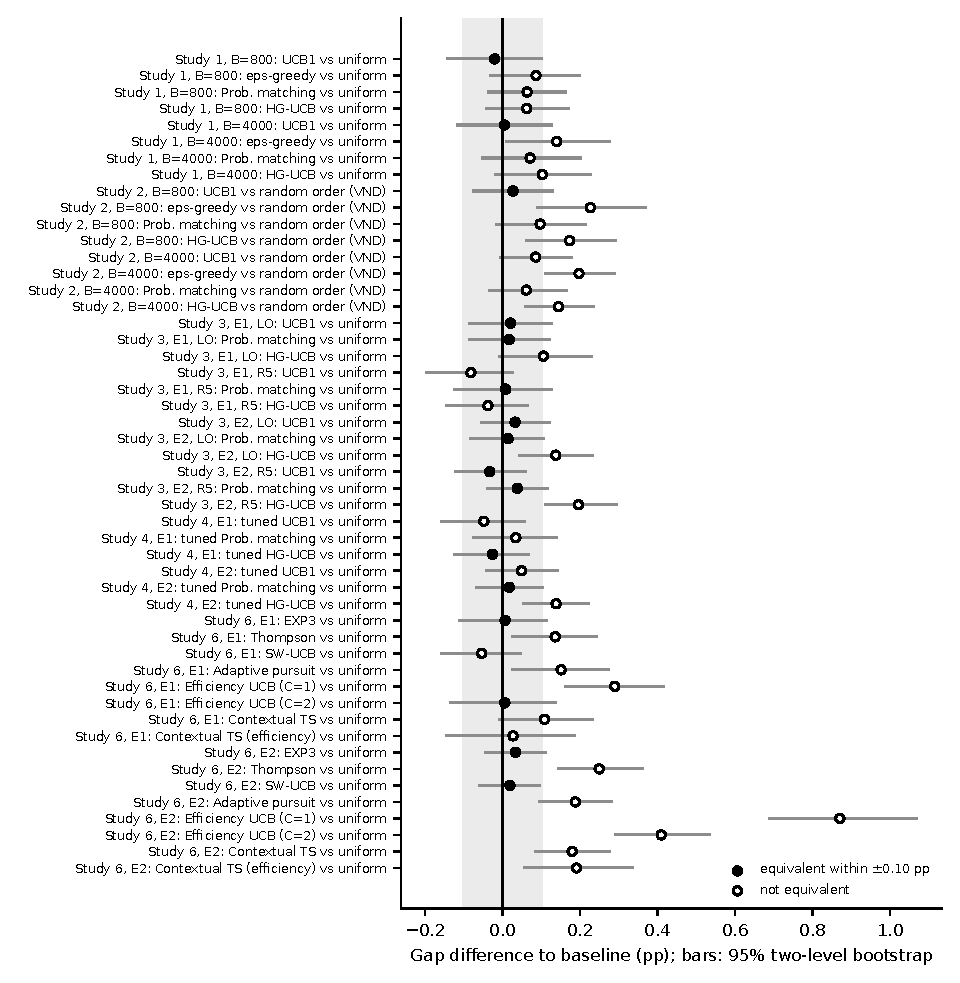
\includegraphics[width=0.9\linewidth]{fig_forest.pdf}
\caption{Equivalence audit: gap difference between each adaptive policy and its baseline in Studies 1--4 and 6. Filled markers: 90\% interval inside $\pm0.10$~pp (equivalent). Bars: 95\% two-level bootstrap intervals.}\label{fig:forest}
\end{figure}

\subsection{Reference ceiling and context}\label{sec:ceiling}
For context, HGS-CVRP \citep{vidal2022}, given the same wall-clock budget as our VNS (\num{hgs_matched_t_min}--\num{hgs_matched_t_max}~s per instance), reaches a mean gap of \num{hgs_matched}\% on the 74 instances, and \num{hgs_n01}\% with 0.1~s per customer, against \num{vns_gap_min}--\num{vns_gap_max}\% for the (non-literal) VNS variants studied here. Part of this distance is implementation language (C++ against Python), so we claim no ranking, only that no variant studied is competitive with the state of the art. An attention-based constructive model \citep{kool2019} used zero-shot reaches a mean gap of \num{kool_gap}\% over the 74 instances when the route-count constraint is ignored (\num{kool_gap_strict}\% on the \num{kool_nstrict} instances that satisfy it).